\documentclass[aspectratio=169]{beamer}
\usetheme{Madrid}
\usepackage[utf8]{inputenc}
\usepackage[T1]{fontenc}
\usepackage{tikz}
\usepackage{amssymb}
\usepackage{graphicx}
\setbeamertemplate{navigation symbols}{}
\setbeamercolor{title}{fg=white,bg=green!55!teal}
\setbeamercolor{frametitle}{fg=white,bg=green!55!teal}
\setbeamercolor{block title}{bg=green!55!teal!20,fg=black}
\setbeamercolor{block body}{bg=green!55!teal!8,fg=black}
\setbeamercolor{item}{fg=green!55!teal}
\setbeamercolor{itemize item}{fg=green!55!teal}
\setbeamertemplate{itemize item}[triangle]

\title{M8 — The Connected World}
\subtitle{How the internet works, staying safe, a one-page HTML profile}
\author{ByteForge --- Grade 8 --- App Builder}
\date{}

\begin{document}

\begin{frame}
    \titlepage
\end{frame}

\begin{frame}{Today's Plan}
    \begin{itemize}
        \item Packets
        \item Generating HTML with Python
        \item Password Strength
        \item https:// vs. http://
        \item Linking Pages
        \item[$\bigstar$] BOSS --- M8 Capstone
    \end{itemize}
\end{frame}

\begin{frame}{Packets — messages arrive out of order}
    \large
    \begin{itemize}
        \item A message is split into packets, sent separately, and can arrive in ANY order
        \item Sorting them back into place by index is exactly what the real internet's TCP protocol does constantly.
    \end{itemize}
\end{frame}


\begin{frame}{Generating real HTML with Python}
    \large
    \begin{itemize}
        \item Every website is really a plain text file written in HTML
        \item Servers routinely BUILD that text on the fly using a real programming language.
    \end{itemize}
\end{frame}


\begin{frame}{Password strength — combining checks in a function}
    \large
    \begin{itemize}
        \item \texttt{is\_strong(password)} returns True only when BOTH the length check AND the digit check pass
        \item \texttt{and} requires every condition to be true.
    \end{itemize}
\end{frame}


\begin{frame}{https:// vs. http:// — a real security check}
    \large
    \begin{itemize}
        \item \texttt{url.startswith("https://")} checks the connection is encrypted
        \item Without it, anything typed (including passwords) travels unprotected.
    \end{itemize}
\end{frame}

\begin{frame}{Real-World Examples}
    \large
    \begin{itemize}
        \item Every online payment, every login form, depends on that padlock/https check being real
        \item This chapter writes the exact check your own browser performs automatically, every single page load.
    \end{itemize}
\end{frame}


\begin{frame}{Image}
    \begin{center}
    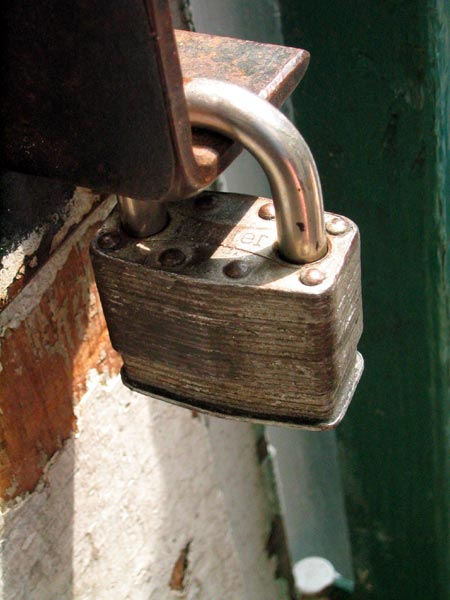
\includegraphics[width=0.5\textwidth]{images/padlock.jpg}

    \large What https:// actually protects --- this chapter's real security check.

    \small Padlock — Alyson Hurt, CC BY 2.0, via Wikimedia Commons
    \end{center}
\end{frame}

\begin{frame}{Let Them Discover}
    \Large
    Check the address bar on 3 different real websites you use. Do they all start with https://? What would you do differently on a page that only had http://?
\end{frame}

\begin{frame}{Your Turn}
    \Large
    Open the student map, find \textbf{M8 — The Connected World}, and work through it
    hands-on --- everything you just saw, they now do themselves.
\end{frame}

\end{document}
